%!TEX root = ../paper.tex
\begin{subfigure}{0.18\textwidth}
	\centering
	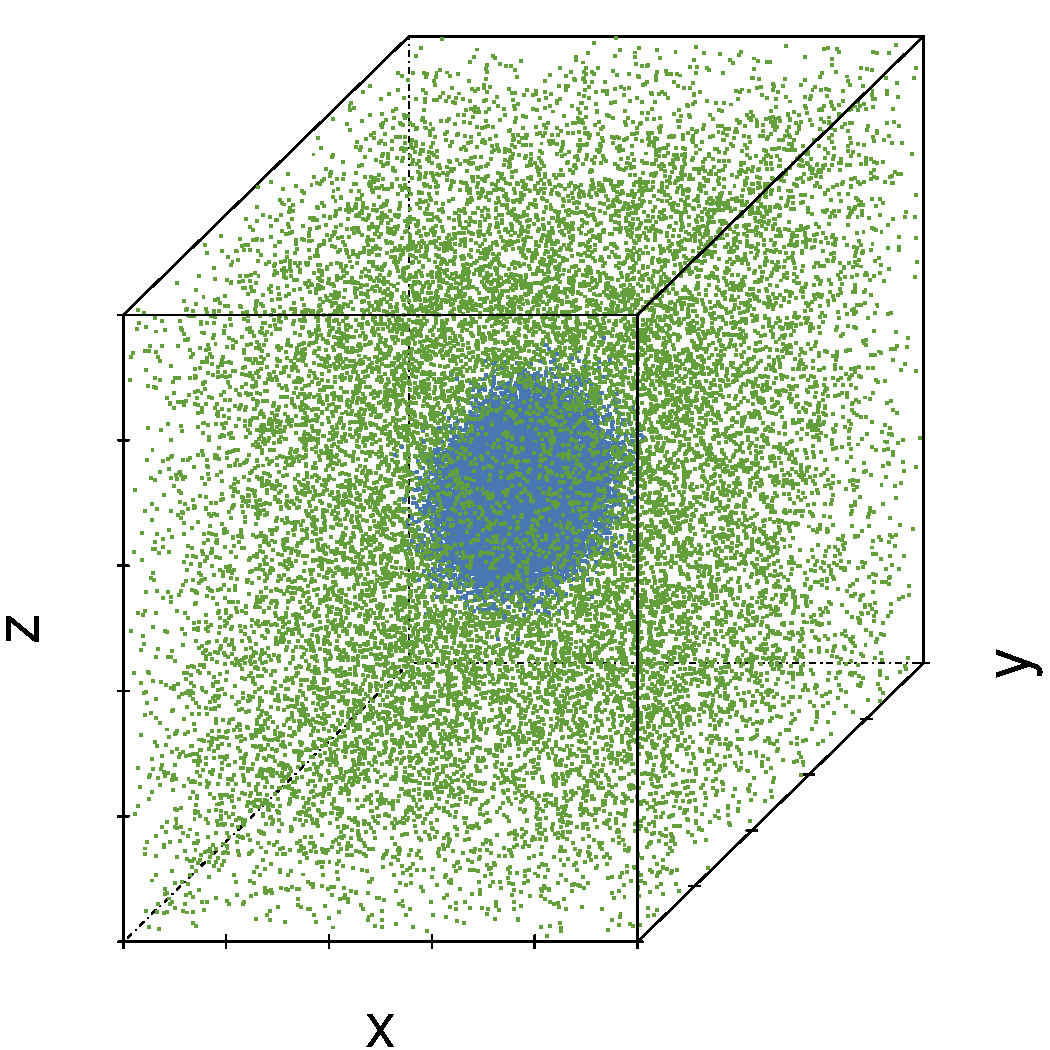
\includegraphics[width=\textwidth]{3/img/datasetplot_ferdosi_1_60000.pdf}
	\caption{Set 1}
	\label{fig:3:simulated:datasets:ferdosi1}
\end{subfigure}
\begin{subfigure}{0.18\textwidth}
	\centering
	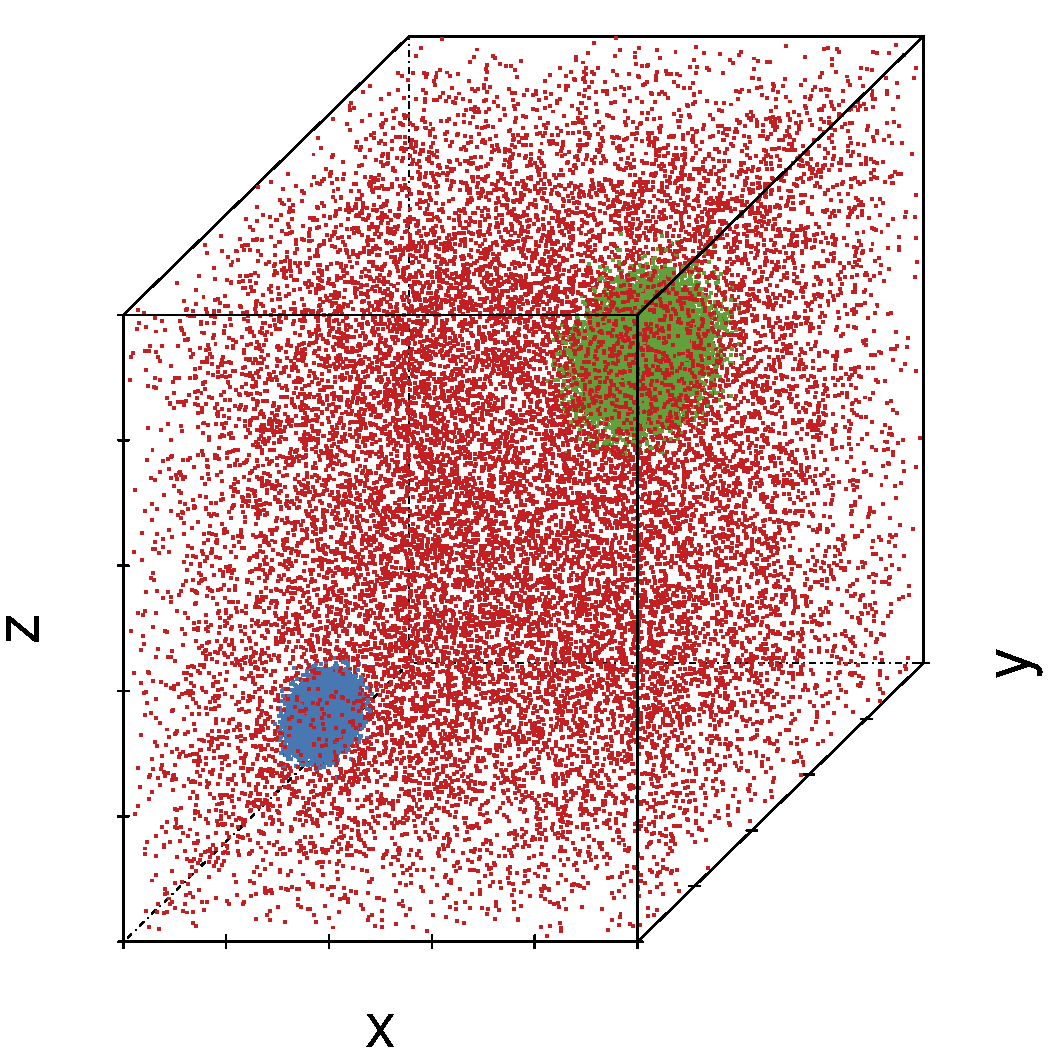
\includegraphics[width=\textwidth]{3/img/datasetplot_ferdosi_2_60000.pdf}
	\caption{Set 2}
	\label{fig:3:simulated:datasets:ferdosi2}
\end{subfigure}	
\begin{subfigure}{0.18\textwidth}
	\centering
	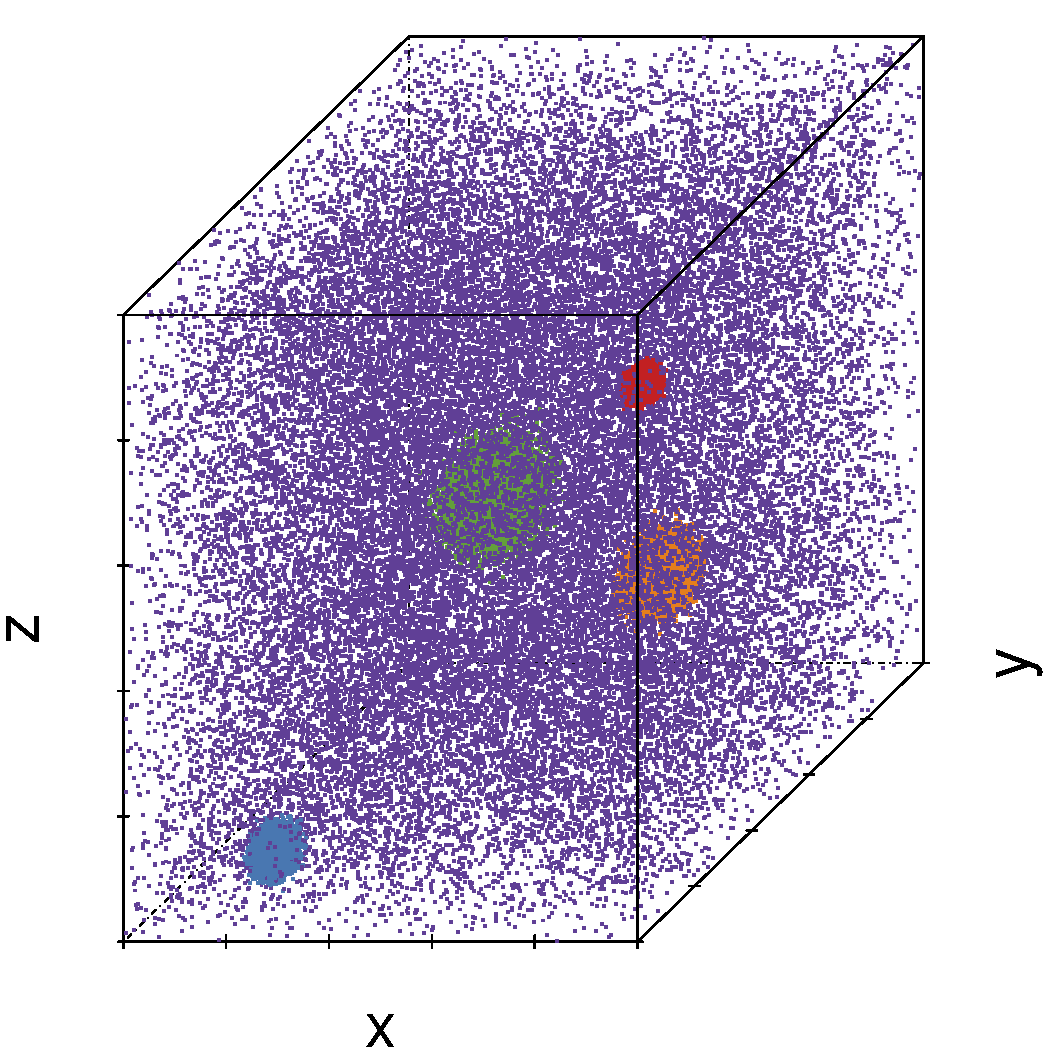
\includegraphics[width=\textwidth]{3/img/datasetplot_ferdosi_3_120000.pdf}
	\caption{Set 3}
	\label{fig:3:simulated:datasets:ferdosi3}
\end{subfigure}		
\begin{subfigure}{0.18\textwidth}
	\centering
	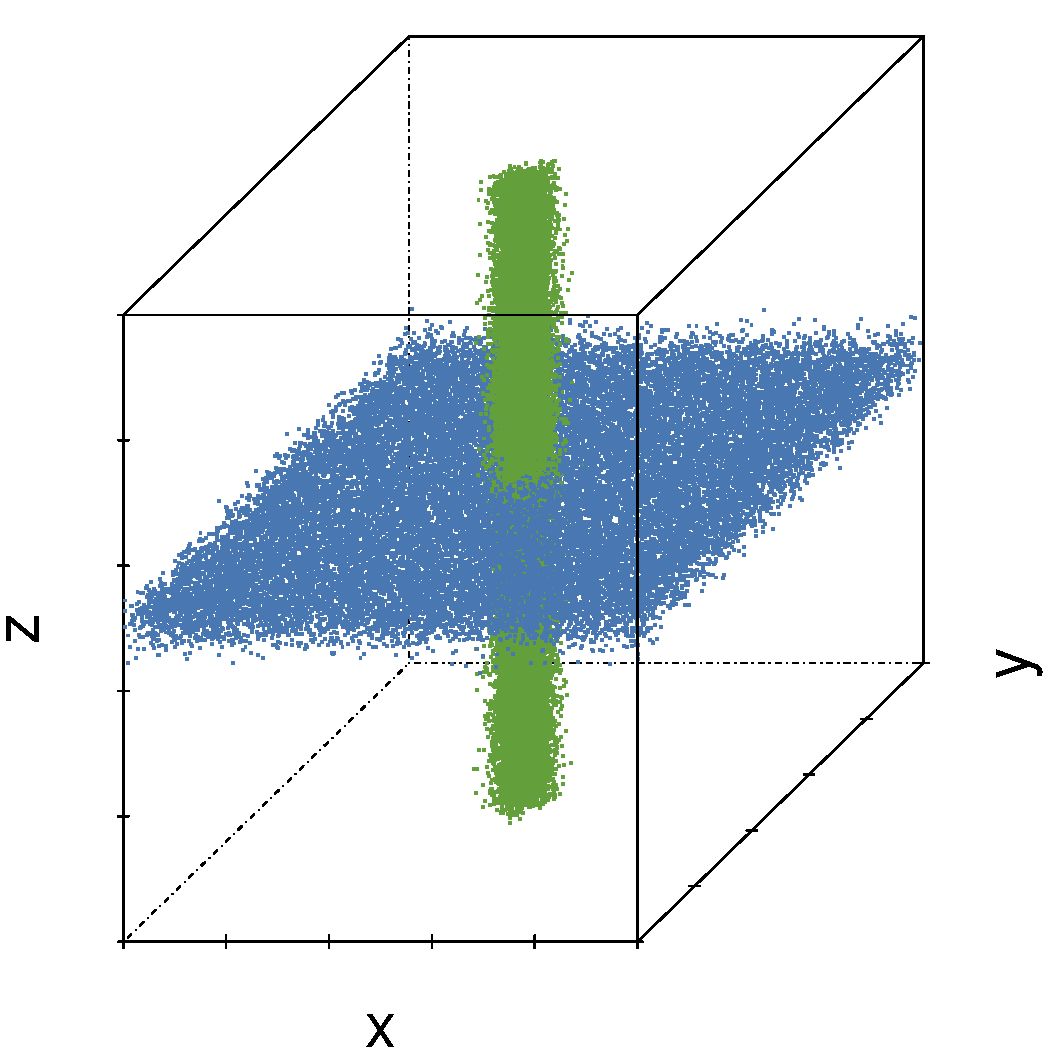
\includegraphics[width=\textwidth]{3/img/datasetplot_ferdosi_4_60000.pdf}
	\caption{Set 4}
	\label{fig:3:simulated:datasets:ferdosi4}
\end{subfigure}			
\begin{subfigure}{0.18\textwidth}
	\centering
	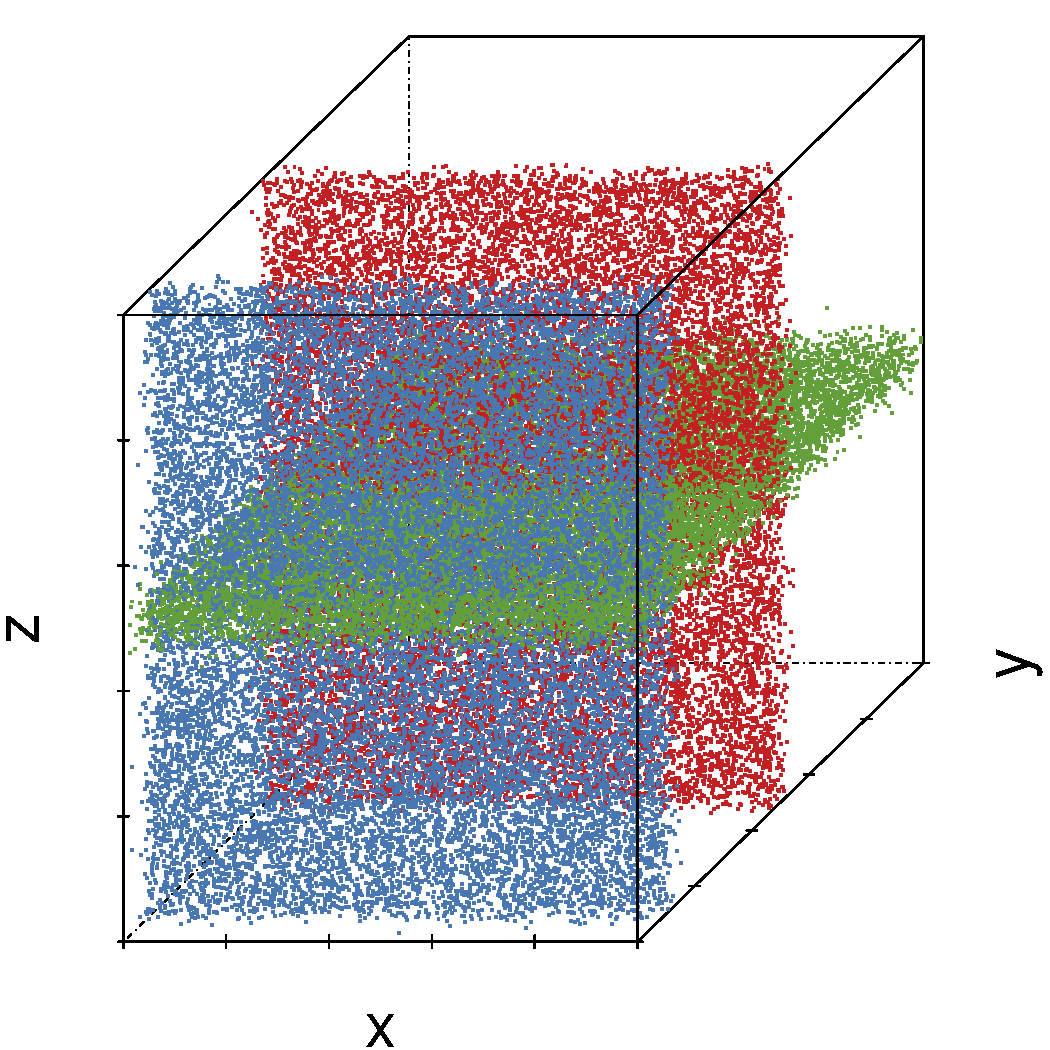
\includegraphics[width=\textwidth]{3/img/datasetplot_ferdosi_5_60000.pdf}
	\caption{Set 5}
	\label{fig:3:simulated:datasets:ferdosi5}
\end{subfigure}	